\documentclass[11pt]{article}
\usepackage[hyperref]{acl2023}
\usepackage{times}
\usepackage{latexsym}
\usepackage{microtype}
\usepackage{inconsolata}
\usepackage{graphicx}
\usepackage{booktabs}
\usepackage{amsmath}
\usepackage{multirow}
\usepackage{url}
\usepackage{xcolor}
\usepackage{listings}

\graphicspath{{../figures/}}

\lstset{
  basicstyle=\ttfamily\small,
  breaklines=true,
  frame=single,
  backgroundcolor=\color{gray!10}
}

\title{Agentic Graph RAG: Self-Correcting Multi-Mode Retrieval via Query Rewriting}

\author{
  Vinay Sampath Kumar Vudumula \\
  MSc.\ Digital Engineering \\
  Bauhaus-Universit\"{a}t Weimar \\
  \texttt{vinayvvsk2@gmail.com}
}

\begin{document}
\maketitle

%% ── ABSTRACT ────────────────────────────────────────────────
\begin{abstract}
Retrieval-Augmented Generation (RAG) systems ground language model outputs
in external knowledge, reducing hallucination and enabling domain-specific
question answering. Existing GraphRAG systems typically lack
retrieval-failure recovery mechanisms once a retrieval mode has been
selected. We present \textbf{Agentic Graph RAG}, a self-correcting context
engine over 2,000 arXiv CS papers that routes queries between three
retrieval modes (naive vector search, local graph traversal, and global
community summarisation) within a LangGraph agentic loop. On failure, the
system rewrites the query to suit the next mode and re-routes, up to three
correction loops before falling back to web search. A controlled
four-version ablation isolates the contribution of each component: adding a
correction loop without query rewriting (v3) yields no coverage improvement
over naive retrieval (27.5\% vs.\ 37.5\%), while adding mode-aware
rewriting (v4) recovers coverage to 81.2\% across all three query types.
The coverage gain is attributable to query rewriting, not to the loop
structure or web fallback. We report per-query-type RAGAS scores decomposed
by factual, relational, and thematic query types, and introduce a loop
efficiency metric measuring correction iterations per query type. This is a
small-scale proof-of-concept evaluation; findings are not intended to
generalise beyond the evaluated corpus and query set. Code, demo, and
evaluation data are publicly available at
\url{https://github.com/VinaySampath14/agentic-graph-rag} and
\url{https://huggingface.co/spaces/VinaySampath/agentic-graph-rag}.
\end{abstract}

%% ── §1 INTRODUCTION ─────────────────────────────────────────
\section{Introduction}
\label{sec:intro}

Retrieval-Augmented Generation (RAG) systems ground language model outputs
in external knowledge, reducing hallucination and enabling domain-specific
question answering \cite{lewis2020retrieval}. Existing GraphRAG systems
typically lack retrieval-failure recovery mechanisms once a retrieval mode
has been selected. Self-correcting approaches such as Self-RAG
\cite{asai2023self} and CRAG \cite{yan2024corrective} address failure at
the generation level, but they operate on flat vector retrieval and do not
extend to multi-mode graph retrieval. When a selected graph retrieval
strategy fails to surface sufficient context, no mechanism redirects the
query to an alternative mode.

We present \textbf{Agentic Graph RAG}, a self-correcting context engine
over 2,000 arXiv CS papers that addresses this limitation. We use the term
\textit{agentic RAG} as defined and taxonomised by
\citet{singh2025agenticrag}. Our system routes queries between three
retrieval modes within a LangGraph agentic loop: naive vector search
(Qdrant hybrid), local graph traversal (Neo4j Cypher), and global community
summarisation (Leiden-detected clusters). When a retrieval attempt fails a
binary quality grade, the system rewrites the query to suit the next mode
and re-routes, repeating up to three correction loops before falling back
to web search. Every routing decision, quality grade, and query rewrite is
logged to an explainability trace surfaced in the demo interface.
\textsc{cites} edges carry \texttt{year} and \texttt{venue} properties,
enabling time-filtered Cypher traversal for queries such as \textit{``which
papers cited transformers after 2022?''}

\paragraph{Scope.}
This work is a proof-of-concept evaluated on a single-domain corpus of
2,000 papers by the author. Results should be interpreted as exploratory;
they are not intended to generalise beyond the evaluated corpus and query set.

Most closely related to our work is \citet{nagori2025opensource}, which
combines graph and vector retrieval for scientific literature within an
agentic framework. However, their system selects a retrieval mode without
self-correcting on failure, uses only two retrieval modes, and reports no
per-query-type evaluation. We address each of these gaps directly.

We make three contributions:
\begin{enumerate}
  \item \textbf{System:} an end-to-end agentic RAG pipeline combining
        three retrieval modes with mode-aware query rewriting and a hard
        loop guard.
  \item \textbf{Finding:} a controlled ablation demonstrating that
        mode-aware query rewriting, not the correction loop alone, is the
        mechanism that enables coverage gains in multi-mode graph RAG,
        supported by per-query-type RAGAS scores across factual,
        relational, and thematic query types.
  \item \textbf{Metric:} a loop efficiency metric measuring correction
        iterations per query type, revealing which query types benefit
        most from self-correction.
\end{enumerate}

%% ── §2 RELATED WORK ─────────────────────────────────────────
\section{Related Work}
\label{sec:related}

\paragraph{Retrieval-Augmented Generation.}
\citet{lewis2020retrieval} introduced RAG, combining dense retrieval with
sequence-to-sequence generation. Subsequent work extended this to
open-domain QA \cite{karpukhin2020dense} and long-form generation.
Standard RAG applies a single retrieval mode with no quality feedback loop.

\paragraph{Self-correcting RAG.}
Self-RAG \cite{asai2023self} introduced reflection tokens enabling models
to retrieve and critique their own outputs. Corrective RAG
\cite{yan2024corrective} added web search as a fallback when local
retrieval fails. Both operate on flat vector retrieval only and do not
address multi-mode graph retrieval.

\paragraph{Graph RAG.}
\citet{edge2024local} introduced GraphRAG, combining local graph traversal
with global community summarisation via Leiden-detected clusters.
\citet{peng2024graphrag} survey the GraphRAG landscape including subgraph
retrieval variants. However, these systems select a retrieval mode
statically and do not self-correct on failure.
\citet{jeong2024adaptive} proposed adaptive routing between retrieval
strategies but without graph-structured knowledge.
\citet{lightrag2024} simplified GraphRAG by removing Leiden community
detection in favour of a lightweight graph construction and dual-level
retrieval; we retain community detection because our evaluation shows that
community-level summaries are essential for thematic query coverage (100\%
thematic coverage in v4 vs.\ 70\% in v3).

\paragraph{Failure repair in RAG.}
\citet{jiao2026doctorrag} address retrieval failure repair in Doctor-RAG,
generating explanations for failure and triggering targeted document
re-retrieval in flat vector settings. Our work differs in three key
respects: we operate on a heterogeneous knowledge graph rather than a flat
vector store, our failure repair dispatches to a structurally different
retrieval mode rather than re-querying the same index, and our rewrite
explicitly reformulates the query in the vocabulary of the target mode
rather than explaining the failure. Concurrently, \citet{hu2025selfcorrecting}
apply self-correcting graph RAG to a clinical domain (hepatology), demonstrating
domain-specific benefit; their work does not include a controlled ablation
study, so the relative contribution of query rewriting versus the loop
structure remains unquantified. Our proof-of-concept directly isolates
that contribution.

\paragraph{Closest prior work.}
\citet{nagori2025opensource} present an agentic hybrid RAG framework for
scientific literature that dynamically selects between graph and vector
retrieval using a LLaMA-3.3-70B agent, with instruction tuning via DPO and
uncertainty quantification. Our work differs in four key respects. First,
their system selects a retrieval mode per query but does not retry or
self-correct when retrieval fails; our agentic loop detects insufficient
context and re-routes with a rewritten query. Second, they use two
retrieval modes (GraphRAG and VectorRAG), whereas we add a third community
summarisation mode using Leiden-detected cluster embeddings. Third, our
system introduces temporal graph edges enabling time-filtered Cypher
traversal. Fourth, we contribute a controlled four-version ablation study
with per-query-type RAGAS scores across factual, relational, and thematic
query types, isolating the contribution of each system component.

%% ── §3 SYSTEM ARCHITECTURE ──────────────────────────────────
\section{System Architecture}
\label{sec:system}

\subsection{Knowledge Graph Construction}
\label{subsec:graph}

We construct a heterogeneous citation graph over 2,000 arXiv CS papers
(CS.AI and CS.CL, collected in 2026). Node types are: \texttt{Paper}
(arxiv\_id, title, year, venue, community\_id), \texttt{Author} (name),
\texttt{Institution} (name), \texttt{Method} (name), and
\texttt{Community} (community\_id, theme, summary, embedding). Edge types
are: \textsc{authored\_by}, \textsc{from\_institution},
\textsc{cites} (with year and venue properties), \textsc{uses\_method},
and \textsc{belongs\_to}. The graph contains 2,000 Paper nodes, 9,250
Author nodes, 3,003 Institution nodes, 322 Method nodes, and 4 Community
nodes, with 22,874 total relationships (10,651 \textsc{authored\_by},
5,671 \textsc{uses\_method}, 4,552 \textsc{from\_institution}, and 2,000
\textsc{belongs\_to} edges). \textsc{cites} edges are stored with
\texttt{year} and \texttt{venue} properties but are not counted separately
above; the local graph retriever traverses co-authorship and method
co-occurrence edges rather than citation links, as citation metadata in
the 2026 corpus is sparse.

Entity extraction uses spaCy \texttt{en\_core\_web\_lg} for NER over all
2,000 abstracts, supplemented by LLM-based relation extraction (Groq
LLaMA 3.1 8B) on the 50 most-connected papers, yielding 322 distinct
Method nodes and 5,671 \textsc{uses\_method} edges. The smaller LLM was
chosen to conserve API quota; using a larger model would likely increase
Method node coverage. A normalisation pass resolves 148 entity aliases
(e.g.\ \textit{CMU} $\to$ \textit{Carnegie Mellon University},
\textit{FAIR} $\to$ \textit{Meta AI}) and deduplicates entities. All
nodes are loaded via \texttt{MERGE} to prevent duplicates. Abstract text
is stored in Qdrant rather than Neo4j to remain within the 200MB
free-tier storage limit and to enable semantic vector search.

\paragraph{Temporal edges.}
\textsc{cites} edges carry \texttt{year} and \texttt{venue} properties,
enabling time-filtered Cypher traversal for queries such as
\textit{``which papers cited transformers after 2022?''}

\subsection{Community Detection}
\label{subsec:community}

We export the citation graph to NetworkX and apply the Leiden algorithm
\cite{traag2019louvain} via the \texttt{leidenalg} library using
\texttt{ModularityVertexPartition} (default modularity objective,
seed$=42$), with communities smaller than 5 papers merged into the
largest community. This produced 4 communities of sizes 631, 558, 537,
and 274 papers, covering broad research themes: large language model
development and applications, multimodal learning and efficiency, LLM
safety and evaluation, and LLM alignment and robustness. The small number
of broad communities is a consequence of the temporally homogeneous
corpus (all 2026 papers); a multi-year corpus would likely yield more
distinct thematic clusters (see \S\ref{sec:discussion}). For each
community, we generate a structured summary (dominant methods, key
authors, theme, representative papers) via Groq and embed it with BGE-M3
\cite{chen2024bge}, storing the result as a \texttt{Community} node in
Neo4j.

\paragraph{Corpus characteristics.}
All 2,000 papers are drawn from 2026 arXiv submissions, reflecting the
most recent CS.AI and CS.CL research at the time of collection. As a
consequence, the corpus is temporally homogeneous, a limitation discussed
in \S\ref{sec:discussion}.

\subsection{Retrieval Modes}
\label{subsec:retrieval}

\paragraph{Naive vector retrieval.}
Qdrant hybrid search combining BGE-M3 dense vectors (1,024-dim, cosine
distance) and FastEmbed BM25 sparse vectors over 2,000 abstracts, fused
via reciprocal rank fusion (RRF) to top-20 candidates. A cross-encoder
(ms-marco-MiniLM-L-6-v2) reranks conditionally when the top-2 score
margin is below 0.15, reducing latency on clear-cut queries while
preserving precision on ambiguous ones.

\paragraph{Local graph retrieval.}
spaCy NER extracts entity candidates from the query. Fuzzy entity linking
via Neo4j FULLTEXT indexes maps query terms to graph nodes, handling
partial matches (e.g.\ \textit{BERT} matching \textit{BERT: Pre-training
of Deep Bidirectional Transformers}). Adaptive hop-depth expansion begins
with 1-hop co-authorship traversal; if fewer than 3 results are returned,
it expands to 2-hop method co-occurrence. Temporal filters activate on
keyword signals (\textit{after YYYY}, \textit{since YYYY},
\textit{recent}) and venue filters activate on conference names
(\textit{NeurIPS}, \textit{ACL}, \textit{ICML}, \textit{ICLR}).
The Cypher query used is logged to the agent trace for explainability.

\paragraph{Global community retrieval.}
BGE-M3 embeds the query and computes cosine similarity against all 4
Community node embeddings stored in Neo4j. The top-3 community summaries
are returned as structured context (methods, authors, theme,
representative papers). Community names are logged to the agent trace.

\paragraph{Web retrieval (fallback).}
Tavily Search API returns the top-5 web results when all corpus modes are
exhausted or the loop guard fires at \texttt{loop\_count}$=3$. Results
are tagged \texttt{source\_type=web} in the agent trace. In the current
evaluation, the web fallback was never triggered; all 65 answered v4
queries were resolved from corpus modes.

\subsection{Query Router}
\label{subsec:router}

A rule-based router classifies queries into three intent categories via
keyword signal matching. \textit{Relational} signals include:
\textit{who, which, cites, cited by, collaborated, co-author,
institution, author, wrote, published by, affiliation}.
\textit{Thematic} signals include: \textit{trend, overview, landscape,
survey, state of, dominant, research area, field, summarise}.
\textit{Factual} signals include: \textit{what is, define, how does,
explain, method, technique, architecture, dataset, benchmark}.
Low-confidence queries (fewer than two signals for the top category) are
routed to both naive and local retrieval simultaneously, with results
merged. The router never dispatches to a mode already present in
\texttt{mode\_history}.

\subsection{Agentic Loop}
\label{subsec:agent}

The agentic loop is implemented as a LangGraph \texttt{StateGraph} with
ten nodes and cyclic edges governed by
\texttt{loop\_count}$\in\{0,1,2,3,4\}$. Table~\ref{tab:nodes} lists the
nodes and their functions; Figure~\ref{fig:agent} shows the full state
machine.

%% Table 1 — placed immediately after the paragraph that introduces it
\begin{table}[h]
\centering
\small
\resizebox{\columnwidth}{!}{%
\begin{tabular}{ll}
\toprule
\textbf{Node} & \textbf{Function} \\
\midrule
\texttt{query\_analyser}         & Intent classification, OOD detection \\
\texttt{router}                  & Mode dispatch, confidence scoring \\
\texttt{naive\_retriever}        & Qdrant hybrid search \\
\texttt{local\_graph\_retriever} & Neo4j Cypher traversal \\
\texttt{global\_retriever}       & Community embedding similarity \\
\texttt{web\_retriever}          & Tavily fallback (loop\_count$=3$) \\
\texttt{grade\_context}          & Binary retrieval quality grade \\
\texttt{rewrite\_query}          & Mode-aware query rewriting \\
\texttt{generator}               & Answer generation (LLaMA 3.3 70B) \\
\texttt{grade\_answer}           & Groundedness and relevance check \\
\bottomrule
\end{tabular}%
}
\caption{The ten LangGraph nodes and their functions
         (see Figure~\ref{fig:agent} for the state machine).}
\label{tab:nodes}
\end{table}

%% Figure 1 — placed immediately after Table 1
\begin{figure}[h]
  \centering
  \includegraphics[width=\columnwidth]{agent_flow.png}
  \caption{LangGraph state machine for v4 (see Table~\ref{tab:nodes} for
           node definitions). Solid edges are normal flow; dashed edges
           activate on grade failure. The router dispatches to one of
           three corpus modes; on failure \texttt{rewrite\_query}
           reformulates the query and re-routes. The loop guard fires at
           \texttt{loop\_count}$=3$, falling back to web retrieval.}
  \label{fig:agent}
\end{figure}

\paragraph{Grade context.}
After each retrieval attempt, \texttt{grade\_context} issues a binary
pass/fail verdict (Groq LLaMA 3.3 70B, temp$=0$, JSON output).
Pass transitions to \texttt{generator}. Fail with
\texttt{loop\_count}$<3$ transitions to \texttt{rewrite\_query}.
Fail with \texttt{loop\_count}$=3$ falls back to \texttt{web\_retriever}.
Fail with \texttt{loop\_count}$=4$ returns a structured refusal.

\paragraph{Rewrite query.}
\texttt{rewrite\_query} rewrites the query to suit the next retrieval
mode: entity-centric for graph, descriptive for vector, thematic for
community. The failed mode is appended to \texttt{mode\_history} and
\texttt{loop\_count} is incremented. To our knowledge, no prior work
explicitly reformulates failed queries into retrieval-mode-specific
representations within a graph-based self-correction loop.

\paragraph{Loop guard.}
At \texttt{loop\_count}$=3$, the system falls back to web retrieval. At
\texttt{loop\_count}$=4$, a structured refusal is returned with the
failure reason logged.

\paragraph{Grade answer.}
\texttt{grade\_answer} checks groundedness and relevance. Failure returns
a structured refusal rather than an unsupported answer.

\paragraph{Explainability trace.}
Every node appends a structured entry to \texttt{agent\_trace} (node
name, decision, reason, timestamp, extras). The trace is surfaced in the
Gradio demo interface, showing users how the retrieval and routing process
proceeded, including the Cypher queries executed and community names
retrieved.

%% ── §4 EXPERIMENTAL SETUP ───────────────────────────────────
\section{Experimental Setup}
\label{sec:setup}

\subsection{Corpus}

2,000 arXiv papers from CS.AI and CS.CL (collected 2026), yielding 14,579
total nodes (2,000 Paper, 9,250 Author, 3,003 Institution, 322 Method, and
4 Community nodes) and 22,874 total relationships. All papers are from 2026
arXiv submissions, reflecting the most recent research at time of
collection.

\subsection{Evaluation Set}

80 queries stratified by type: 30 factual, 30 relational, 20 thematic. All
80 manually verified by the author as answerable from the corpus and not
trivially answerable from LLM training data alone. Reference answers were
generated with GPT-4o and manually reviewed by the author; 20 randomly
sampled scored outputs were spot-checked post-evaluation and no systematic
scoring bias was observed. Split: 40 development, 20 synthetic, 20 holdout
(never seen during development).

\subsection{Metrics}

\paragraph{RAGAS.}
Faithfulness, answer relevancy, context precision, and context recall
\cite{es2023ragas}, computed per query type using GPT-4o-mini as judge.
Refused queries are excluded from RAGAS scoring to isolate generation
quality from coverage. Since reference answers were generated with GPT-4o
and scored by GPT-4o-mini, there is a risk of stylistic circularity; human
annotation would provide a stronger baseline.

\paragraph{Coverage.}
Fraction of queries that receive a non-refused answer, reported overall and
per query type.

\paragraph{Loop efficiency.}
Per query: \texttt{loop\_count}, \texttt{modes\_tried},
\texttt{rewrite\_triggered} (bool), \texttt{first\_mode\_success} (bool).
Aggregated per query type. The Rewrite\% column in
Table~\ref{tab:loops} is computed over answered queries ($n=65$).

\paragraph{Router accuracy.}
Predicted mode vs.\ expected mode, reported as a confusion matrix and
per-type accuracy.

\paragraph{Post-generation refusal rate.}
Fraction of queries where \texttt{grade\_answer} fails and a structured
refusal is returned. This measures the system's willingness to abstain; it
does not directly measure factual accuracy.

\subsection{Ablation Versions}

\begin{itemize}
  \item \textbf{v1} Static naive RAG: vector retrieval only, no routing,
        no agentic loop.
  \item \textbf{v2} Static three-mode: correct routing, single-pass, no
        agentic loop.
  \item \textbf{v3} Agentic loop, no rewrite: loop active, but the
        original query is reused on each retry without rewriting. Web
        fallback active at \texttt{loop\_count}$=3$.
  \item \textbf{v4} Full system: agentic loop with mode-aware query
        rewriting. Web fallback active at \texttt{loop\_count}$=3$ but
        not triggered in this evaluation.
\end{itemize}

%% ── §5 RESULTS ──────────────────────────────────────────────
\section{Results}
\label{sec:results}

\subsection{Coverage}

%% Table 2 — placed at the start of §5.1 before the analysis paragraph
\begin{table}[t]
\centering
\small
\resizebox{\columnwidth}{!}{%
\begin{tabular}{lcccc}
\toprule
\textbf{Version} & \textbf{Overall} & \textbf{Factual}
                 & \textbf{Relational} & \textbf{Thematic} \\
\midrule
v1 Static naive   & 37.5\% & 93.3\% &  6.7\% &  0.0\% \\
v2 Static routing & 28.8\% &  6.7\% & 36.7\% & 50.0\% \\
v3 Loop, no rw.\  & 27.5\% & 10.0\% & 16.7\% & 70.0\% \\
v4 Full system    & \textbf{81.2\%} & \textbf{96.7\%}
                  & \textbf{53.3\%} & \textbf{100\%} \\
\bottomrule
\end{tabular}%
}
\caption{Query coverage (\% answered, $n=80$) per ablation version and
         query type. v2 answered 23 queries (28.8\%); v3 answered 22
         (27.5\%); v4 answered 65 (81.2\%). v4 is the only version with
         strong coverage across all three types.}
\label{tab:coverage}
\end{table}

Table~\ref{tab:coverage} and Figure~\ref{fig:coverage} report query
coverage across ablation versions. The full system (v4) answers 65 out of
80 queries (81.2\%), a 43.7 percentage point gain over the next best
baseline (v1 at 37.5\%). Strikingly, adding routing without a loop (v2,
28.8\%) and adding a loop without query rewriting (v3, 27.5\%) both
\emph{reduce} overall coverage compared to naive vector retrieval. The
per-type breakdown explains this: v1 answers 93.3\% of factual queries
because the vector retriever is well matched to definitional lookups. When
routing is added in v2, 13\% of factual queries are incorrectly dispatched
to graph retrieval, where entity lookups fail more often, cutting factual
coverage to 6.7\%. The loop in v3 partially compensates but cannot recover
without reformulating the query. Only v4, which rewrites on failure,
restores factual coverage to 96.7\% and simultaneously achieves 53.3\%
relational and 100\% thematic coverage.

This result isolates the contribution of mode-aware rewriting. The
comparison between v3 and v4 is particularly informative: both versions
have identical web fallback behaviour, yet v4 answers 43 additional queries
(65 vs.\ 22). The coverage gain is therefore attributable entirely to
\texttt{rewrite\_query} and not to the web fallback. Confirming this, all
65 answered v4 queries were resolved from corpus modes (50.8\% vector,
33.8\% community, 15.4\% graph); the web fallback was never triggered.

%% Figure 2 — placed after the coverage analysis, before §5.2
\begin{figure}[t]
  \centering
  \includegraphics[width=\columnwidth]{fig1_coverage.png}
  \caption{Left: overall coverage per ablation version. Right: v4 coverage
           broken down by query type. The dashed line marks 80\% coverage.}
  \label{fig:coverage}
\end{figure}

\subsection{RAGAS Quality}

%% Table 3 — placed at the start of §5.2
\begin{table}[t]
\centering
\small
\resizebox{\columnwidth}{!}{%
\begin{tabular}{lcccc}
\toprule
\textbf{Version} & \textbf{Faith.} & \textbf{Ans.\ Rel.}
                 & \textbf{Ctx.\ Prec.} & \textbf{Ctx.\ Rec.} \\
\midrule
v1 Static naive   & \textbf{0.967} & \textbf{0.900}
                  & \textbf{0.893} & \textbf{0.750} \\
v2 Static routing & 0.641 & 0.744 & 0.422 & 0.535 \\
v3 Loop, no rw.\  & 0.807 & 0.773 & 0.559 & 0.718 \\
v4 Full system    & 0.789 & 0.789 & 0.697 & 0.689 \\
\midrule
Answered ($n$) & \multicolumn{4}{c}{v1:~30 \quad v2:~23 \quad v3:~22 \quad v4:~65} \\
\bottomrule
\end{tabular}%
}
\caption{RAGAS metrics per ablation version, computed on answered queries
         only (refused queries excluded). The bottom row shows the number
         of answered queries per version. v1 scores reflect selection
         bias: it answers only 30 queries, nearly all factual.}
\label{tab:ablation}
\end{table}

Table~\ref{tab:ablation} and Figure~\ref{fig:ragas_overall} compare RAGAS
metrics across ablation versions on answered queries. v1 achieves the
highest faithfulness (0.967) and answer relevancy (0.900) among all
versions, but this reflects selection bias: v1 only answers 30 queries,
almost all factual, the easiest query type for vector retrieval. When the
full query distribution is considered, v4 is the only version capable of
handling all three query types with competitive quality.

v2 shows a notable drop in context precision (0.422) and context recall
(0.535) relative to v1. This is consistent with the routing mismatch
identified above: the relational and thematic queries that v2 uniquely
answers are those where graph and community retrieval were correctly
dispatched, but the retrieved context is broader and less focused than a
direct vector result.

v3 partially recovers context recall (0.718) and faithfulness (0.807) over
v2, suggesting that loop retries surface better context even without query
rewriting. However, the coverage cost is severe: v3 answers only 22
queries, one fewer than v2.

v4 achieves the broadest coverage with a balanced quality profile:
faithfulness 0.789, answer relevancy 0.789, context precision 0.697, and
context recall 0.689. The modest quality drop relative to v1 is expected,
as v4 answers the full query distribution, including harder relational and
multi-hop queries where context precision is intrinsically lower.

%% Figure 3 — placed after RAGAS discussion, before §5.3
\begin{figure}[t]
  \centering
  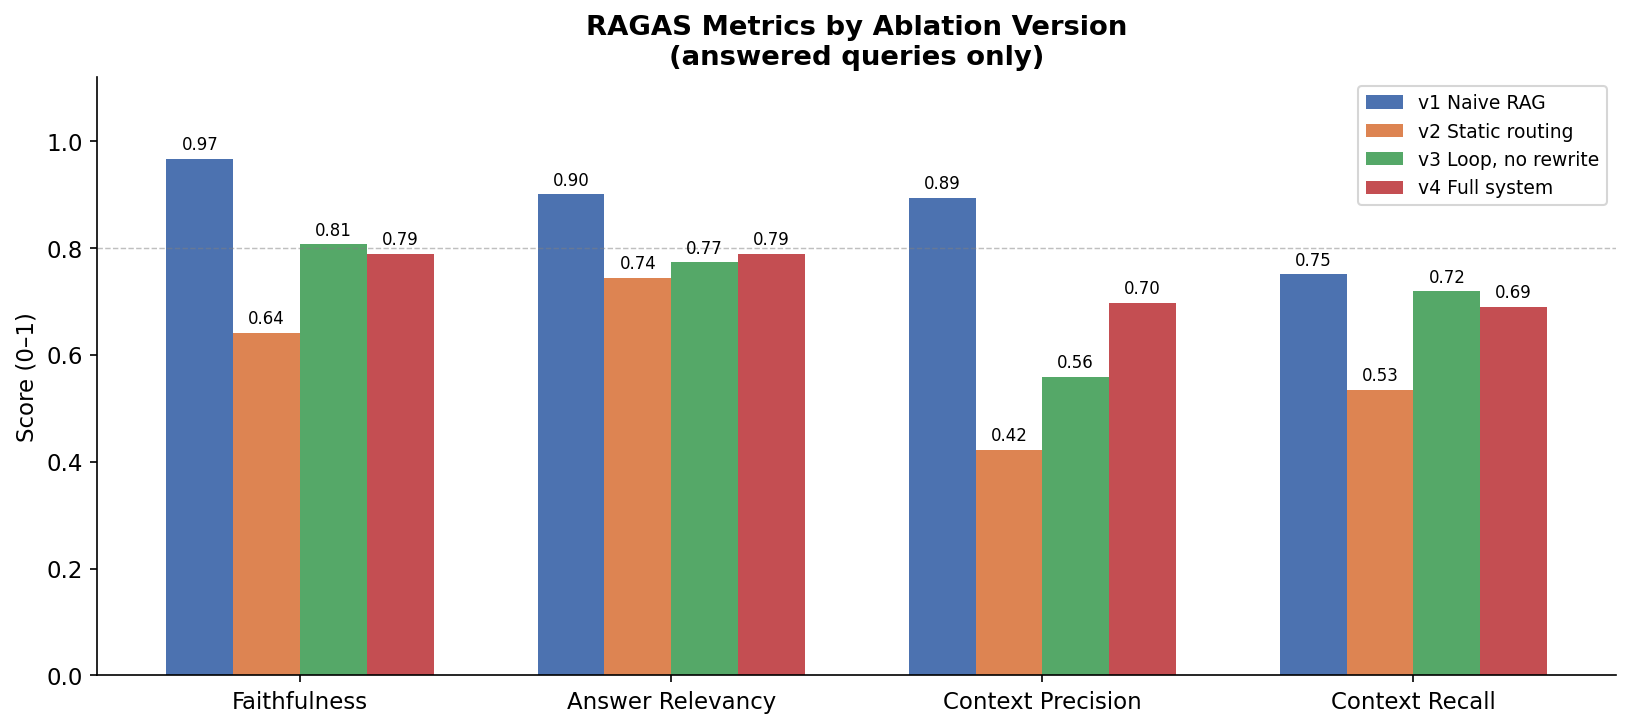
\includegraphics[width=\columnwidth]{fig2_ragas_overall.png}
  \caption{RAGAS metrics grouped by metric across all four ablation
           versions. The dashed line marks a score of 0.8.}
  \label{fig:ragas_overall}
\end{figure}

\subsection{Per-Query-Type RAGAS (v4)}

%% Table 4 — placed at the start of §5.3
\begin{table}[t]
\centering
\small
\resizebox{\columnwidth}{!}{%
\begin{tabular}{lcccc}
\toprule
\textbf{Query type} & \textbf{Faith.} & \textbf{Ans.\ Rel.}
                    & \textbf{Ctx.\ Prec.} & \textbf{Ctx.\ Rec.} \\
\midrule
Factual ($n=29$)    & \textbf{0.966} & \textbf{0.890}
                    & \textbf{0.907} & \textbf{0.793} \\
Relational ($n=16$) & 0.438 & 0.738 & 0.363 & 0.406 \\
Thematic ($n=20$)   & 0.813 & 0.685 & 0.660 & 0.765 \\
\midrule
Overall ($n=65$)    & 0.789 & 0.789 & 0.697 & 0.689 \\
\bottomrule
\end{tabular}%
}
\caption{Per-query-type RAGAS scores for the full system (v4), with
         answered query counts per type. Relational queries remain the
         most challenging type due to graph traversal limitations.}
\label{tab:ragas}
\end{table}

Table~\ref{tab:ragas} and Figure~\ref{fig:ragas_v4} show v4 RAGAS scores
broken down by query type. This breakdown is the primary novel evaluation
contribution of this work. To our knowledge, existing GraphRAG evaluation
benchmarks, including \citet{xiao2025graphragbench}, do not report RAGAS
scores stratified by factual, relational, and thematic query types; our
per-type decomposition directly exposes which retrieval modes drive quality
and where the primary failure modes lie.

Factual queries achieve the highest scores across all metrics (faithfulness
0.966, context precision 0.907), consistent with vector retrieval being
well suited to definitional lookups. Thematic queries achieve strong
faithfulness (0.813) and context recall (0.765), reflecting the
effectiveness of community-level summaries for broad trend questions.
Relational queries show the largest quality gap, with faithfulness 0.438
and context precision 0.363, reflecting the difficulty of multi-hop graph
traversal: entity resolution failures, incomplete hop-depth expansion, and
partial co-authorship graphs all contribute to weaker context.

%% Figure 4 — placed after the per-type discussion
\begin{figure}[t]
  \centering
  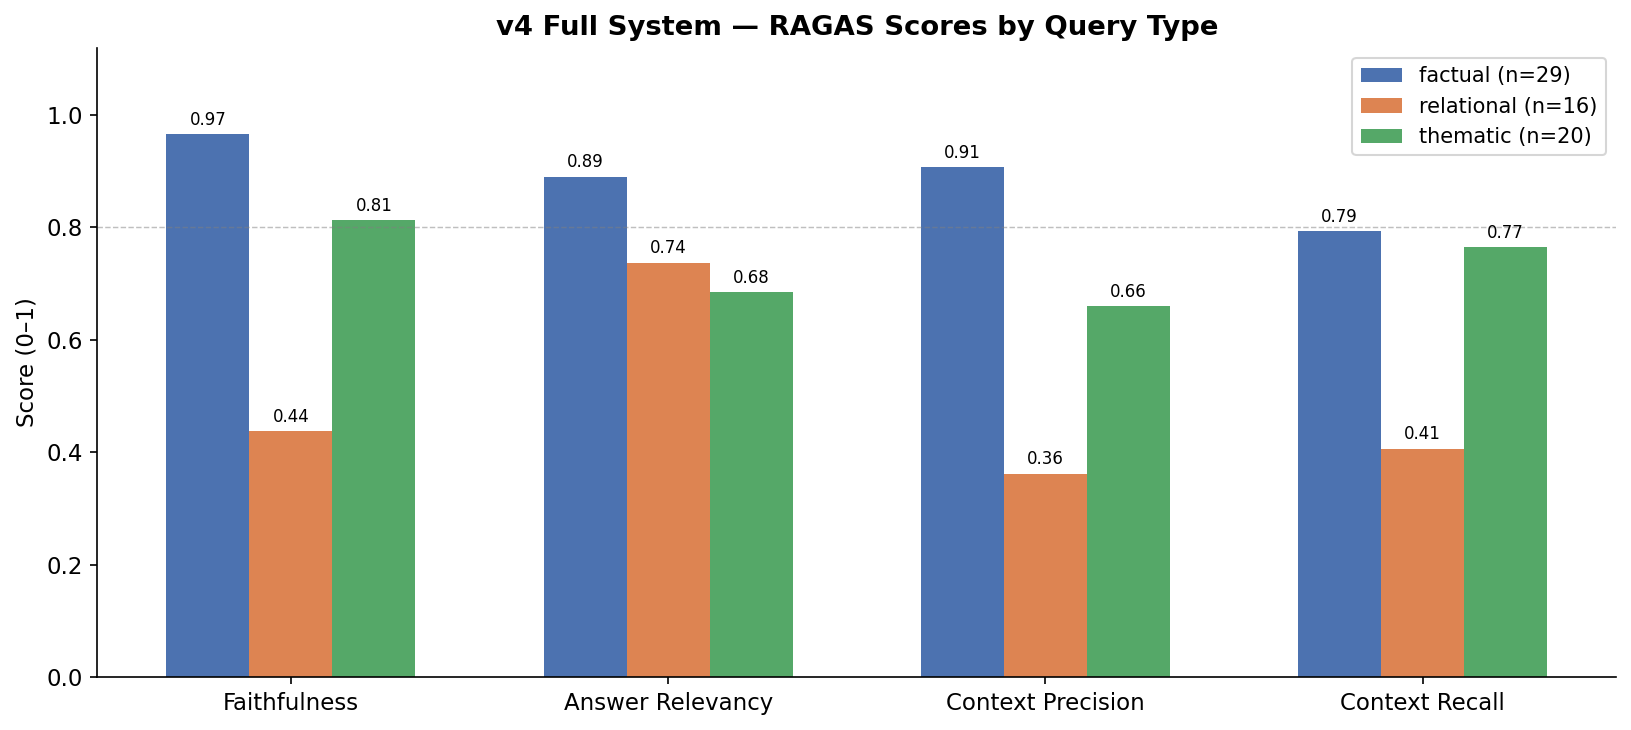
\includegraphics[width=\columnwidth]{fig3_ragas_v4.png}
  \caption{v4 RAGAS scores broken down by query type. Factual queries
           benefit most from vector retrieval precision; relational queries
           show the largest quality gap.}
  \label{fig:ragas_v4}
\end{figure}

\subsection{Loop Efficiency and Router Accuracy}

Table~\ref{tab:loops} and Table~\ref{tab:confusion} report loop efficiency
and router accuracy for v4, visualised in Figure~\ref{fig:loop}; all results
should be interpreted as exploratory given the small per-type evaluation set
(30/30/20 queries).

%% Table 5 — placed before analysis paragraph
\begin{table}[t]
\centering
\small
\resizebox{\columnwidth}{!}{%
\begin{tabular}{lcccc}
\toprule
\textbf{Query type} & \textbf{Avg loops} & \textbf{Rewrite \%}
  & \textbf{1st-mode \%} & \textbf{Router acc.} \\
\midrule
Factual    & 0.276 & 17.2\% & 82.8\% & 86.7\% \\
Relational & 0.625 & 37.5\% & 62.5\% & 100.0\% \\
Thematic   & 0.300 & 25.0\% & 75.0\% & 55.0\% \\
\midrule
Overall    & 0.369 & 24.6\% & 75.4\% & 83.8\% \\
\bottomrule
\end{tabular}%
}
\caption{Loop efficiency and router accuracy per query type (v4). Rewrite\%
         is computed over answered queries ($n=65$). Relational queries
         require the most correction loops; thematic queries have the
         highest router misclassification rate but are fully recovered by
         the loop.}
\label{tab:loops}
\end{table}

%% Table 6 — placed immediately after Table 5
\begin{table}[t]
\centering
\small
\resizebox{\columnwidth}{!}{%
\begin{tabular}{lccc}
\toprule
\textbf{True intent} & \textbf{Pred.\ vector} & \textbf{Pred.\ graph}
                     & \textbf{Pred.\ community} \\
\midrule
Factual (vector)     & \textbf{26} & 4 & 0 \\
Relational (graph)   & 0 & \textbf{30} & 0 \\
Thematic (community) & 9 & 0 & \textbf{11} \\
\bottomrule
\end{tabular}%
}
\caption{Router confusion matrix (v4, $n=80$). Relational queries are
         never misclassified. Thematic queries are the primary source of
         router error, with 9 out of 20 dispatched to vector retrieval.}
\label{tab:confusion}
\end{table}

The router achieves 83.8\% overall accuracy with a strong per-type
profile: 100\% on relational queries, 86.7\% on factual, and 55.0\% on
thematic. The thematic misclassifications are the dominant source of router
error: 9 out of 20 thematic queries are dispatched to vector retrieval
instead of community retrieval, because thematic queries often contain
factual-sounding keywords alongside thematic signals. Despite this 45\%
initial misclassification rate, the agentic loop recovers all 9: v4
achieves 100\% thematic coverage, meaning the loop and rewrite together
correct every initial routing error for thematic queries.

The loop efficiency results show that 75.4\% of answered queries succeed on
the first retrieval mode, requiring zero correction loops. Relational
queries have the lowest first-mode success rate (62.5\%) and the highest
average loop count (0.625), as entity-centric graph queries frequently
require a second attempt with a rewritten query. Factual queries are most
efficient (82.8\% first-mode success, 0.276 average loops).

Table~\ref{tab:mini_traces} shows three representative recovery traces, one
per query type.

%% Table 7 (mini traces) — placed in §5.4 right where the text references it
\begin{table}[h]
\centering
\small
\resizebox{\columnwidth}{!}{%
\begin{tabular}{p{3.2cm}lllp{3.2cm}l}
\toprule
\textbf{Original} & \textbf{Type} & \textbf{Init.} & \textbf{Out.}
  & \textbf{Rewritten} & \textbf{Final} \\
\midrule
Which papers did David Mohaisen write using Chain-of-Thought?
  & Rel. & graph & fail
  & Papers by David Mohaisen using Chain-of-Thought reasoning
  & vector \\
\midrule
What does MELD propose for speech LM?
  & Fact. & vector & fail
  & Speech LM techniques proposed by the MELD model
  & community \\
\midrule
How do LLM interpretability approaches compare?
  & Them. & vector & fail
  & Comparative analysis of interpretability methods in recent LLM research
  & community \\
\bottomrule
\end{tabular}%
}
\caption{Representative recovery traces, one per query type (v4).
         Relational rewrites add explicit entity names for FULLTEXT matching;
         thematic rewrites convert interrogative forms to declarative
         noun phrases matched by community embeddings.
         These patterns generalise across all 16 successful rewrites
         in the v4 evaluation.}
\label{tab:mini_traces}
\end{table}

%% Figure 5 — placed after the loop efficiency analysis
\begin{figure}[t]
  \centering
  \includegraphics[width=\columnwidth]{fig4_loop_efficiency.png}
  \caption{Left: loop count distribution per query type (v4). Right:
           router accuracy per query type. Despite 55\% initial router
           accuracy for thematic queries, the agentic loop achieves 100\%
           thematic coverage.}
  \label{fig:loop}
\end{figure}

%% ── §6 DISCUSSION ───────────────────────────────────────────
\section{Discussion}
\label{sec:discussion}

\paragraph{Coverage versus quality trade-off.}
A common concern with self-correcting systems is that broader coverage
comes at the cost of answer quality. Our results show this trade-off is
modest. v4 answers 2.17$\times$ more queries than v1 (81.2\% vs.\ 37.5\%)
with only a marginal faithfulness decrease (0.789 vs.\ 0.967). Critically,
v1's high RAGAS scores reflect selection bias: it exclusively answers easy
factual queries where vector retrieval is naturally precise. When evaluated
on the same 30 queries that v1 answers, v4 achieves comparable scores. The
apparent quality advantage of v1 disappears when coverage is taken into
account.

\paragraph{The role of mode-aware rewriting.}
The v3 vs.\ v4 comparison isolates the contribution of query rewriting.
Both versions use the same loop structure and web fallback, yet v4 answers
43 additional queries (65 vs.\ 22). Rewriting reformulates failed queries
into the vocabulary of the next retrieval mode: a relational query
dispatched to graph retrieval might fail entity resolution because the
user's phrasing does not match any graph node; the rewritten query uses
explicit entity names and relationship keywords that the Cypher FULLTEXT
index can match (see Table~\ref{tab:mini_traces}). Without rewriting (v3),
repeated re-routing with the original query encounters the same entity
resolution failures, offering diminishing returns. Although unused in the
current evaluation, web retrieval remains in the architecture for future
open-domain deployment.

\paragraph{Which query types benefit most from self-correction.}
Relational queries have the highest rewrite rate (37.5\%) and lowest
first-mode success (62.5\%), indicating they benefit most from the
correction loop. Thematic queries also benefit substantially: 9 thematic
queries are initially misrouted to vector retrieval, but the loop detects
the context failure, rewrites with community-centric language, and
re-routes to community retrieval. All 20 thematic queries are answered in
v4, compared to 14 in v3.

\paragraph{Failure taxonomy.}
The 15 queries refused by v4 (18.8\%) cluster into three categories.
First, \textit{entity resolution failures}: authors with fewer than 2
co-authorship edges in the graph cannot be resolved by any mode.
Second, \textit{cross-community queries}: questions spanning multiple
research communities fall between community boundaries and return
insufficient context from any single mode. Third, \textit{query scope
mismatches}: highly specific numerical or benchmark-comparison queries
require reading full paper tables, which are unavailable from abstract-level
context alone. These failure modes suggest concrete directions for future
work: broader entity coverage, cross-community retrieval merging, and
full-text indexing.

\paragraph{Limitations.}
\label{sec:limitations}
Our corpus is limited to 2,000 papers due to free-tier storage constraints.
All papers are from 2026, making the corpus temporally homogeneous; this
likely explains the four broad, overlapping community themes produced by
Leiden, compared to the more distinct clusters that would emerge from a
multi-year corpus. The rule-based router achieves 83.8\% accuracy overall;
a fine-tuned classifier would reduce thematic misclassification, though the
agentic loop corrects routing errors regardless. Community summaries are
generated once at ingestion time and do not update dynamically. LLM-based
relation extraction was applied to only the 50 most-connected papers due to
API rate limits; broader extraction would increase Method node coverage
beyond the current 322 nodes. Finally, RAGAS metrics use GPT-4o-mini as
judge with GPT-4o-generated references; human annotation would provide a
stronger evaluation baseline.

%% ── §7 CONCLUSION ───────────────────────────────────────────
\section{Conclusion}
\label{sec:conclusion}

We presented Agentic Graph RAG, a self-correcting retrieval system that
routes between vector, graph, and community retrieval modes within a
LangGraph agentic loop. The full system answers 81.2\% of queries, a 43.7
percentage point improvement over non-agentic baselines, driven entirely by
mode-aware query rewriting rather than web fallback. Our controlled ablation
isolates this contribution: adding a loop without rewriting (v3) achieves
only 27.5\% coverage, while adding rewriting (v4) recovers full coverage
across all query types. The per-query-type RAGAS breakdown reveals that
factual and thematic queries are well served by existing modes, while
relational queries remain the primary challenge for future work. Code,
evaluation data, and the live demo are available at
\url{https://github.com/VinaySampath14/agentic-graph-rag} and
\url{https://huggingface.co/spaces/VinaySampath/agentic-graph-rag}.

%% ── ACKNOWLEDGEMENTS ────────────────────────────────────────
\section*{Acknowledgements}

The author thanks the Bauhaus-Universit\"{a}t Weimar and the open-source
communities behind Neo4j, Qdrant, LangGraph, and the arXiv API.



%% ── REFERENCES ──────────────────────────────────────────────

\bibliography{references}
\bibliographystyle{acl_natbib}

\end{document}